\chapter{2-D. Designer fermion lattices} %~~~~~~~~~~~~~~~~~~~~~~~~~~~~~~~~~~~~~%
\section{The Geometry}
Since we require vacancies to be placed only in hollow positions, its possible placements form a triangular lattice \red{($C_6$ symmetry?)}. By carefully choosing the location of the vacancies, many different meta-lattices may appear.
%The artificial lattices that we can build by choosing the correct placing of the vacancies can form almost all the 2D Bravais lattices. \fref{art_lattices}
%%~~~~~~~~~~~~~~~~~~~~~~~~~~ FIGURE ~~~~~~~~~~~~~~~~~~~~~~~~~%
%\begin{figure}[h!]
%\centering
%\includegraphics{path/to/file.ext}
%\vspace{-5pt}
%\caption{Some examples of the possible artificial lattices}
%\label{art_lattices}
%\end{figure}
%\FloatBarrier
%%~~~~~~~~~~~~~~~~~~~~~~~~~~~~~~~~~~~~~~~~~~~~~~~~~~~~~~~~~~~%
Any structure preserving the $C_6$ symmetry can easily be achieved, but even structures breaking this symmetry are possible. For instance we can place two vacancies forming either a rectangular lattice or a honeycomb lattice. Three vacancies per unit cell allow more complex structures such as the Kagome lattice or the centered rectangular lattice.
Strictly speaking, neither oblique nor square lattice can be exactly reproduced but these two are particular examples of the rectangular lattice, so effectively all the 2D possible lattices can be reproduced % TODO wat?!

\section{Control parameters}


\section{Artificial triangular lattice}
By carefully choosing the placement of the vacancies, different 2D lattices can be designed. The electrically tunable gap as well as the distance among vacancies provide two parameters to design fermion models with the desired parameters.
Almost any lattice is feasible, as illustrative examples we will examine a triangular lattice with different unit cells, i.e., a simple triangular lattice, graphene and the Kagome lattice.

The effective parameters will be tuned by choosing the appropriate distances and angles between vacancies and the corresponding electric field.


The simplest effective lattice that can be designed is a triangular lattice with a single site per unit cell. This lattice appears naturally when we consider only the hollow positions of the upper layer in a graphene bilayer.

%~~~~~~~~~~~~~~~~~~~~~~~~~~ FIGURE ~~~~~~~~~~~~~~~~~~~~~~~~~%
\begin{figure}[h!]
  \centering
  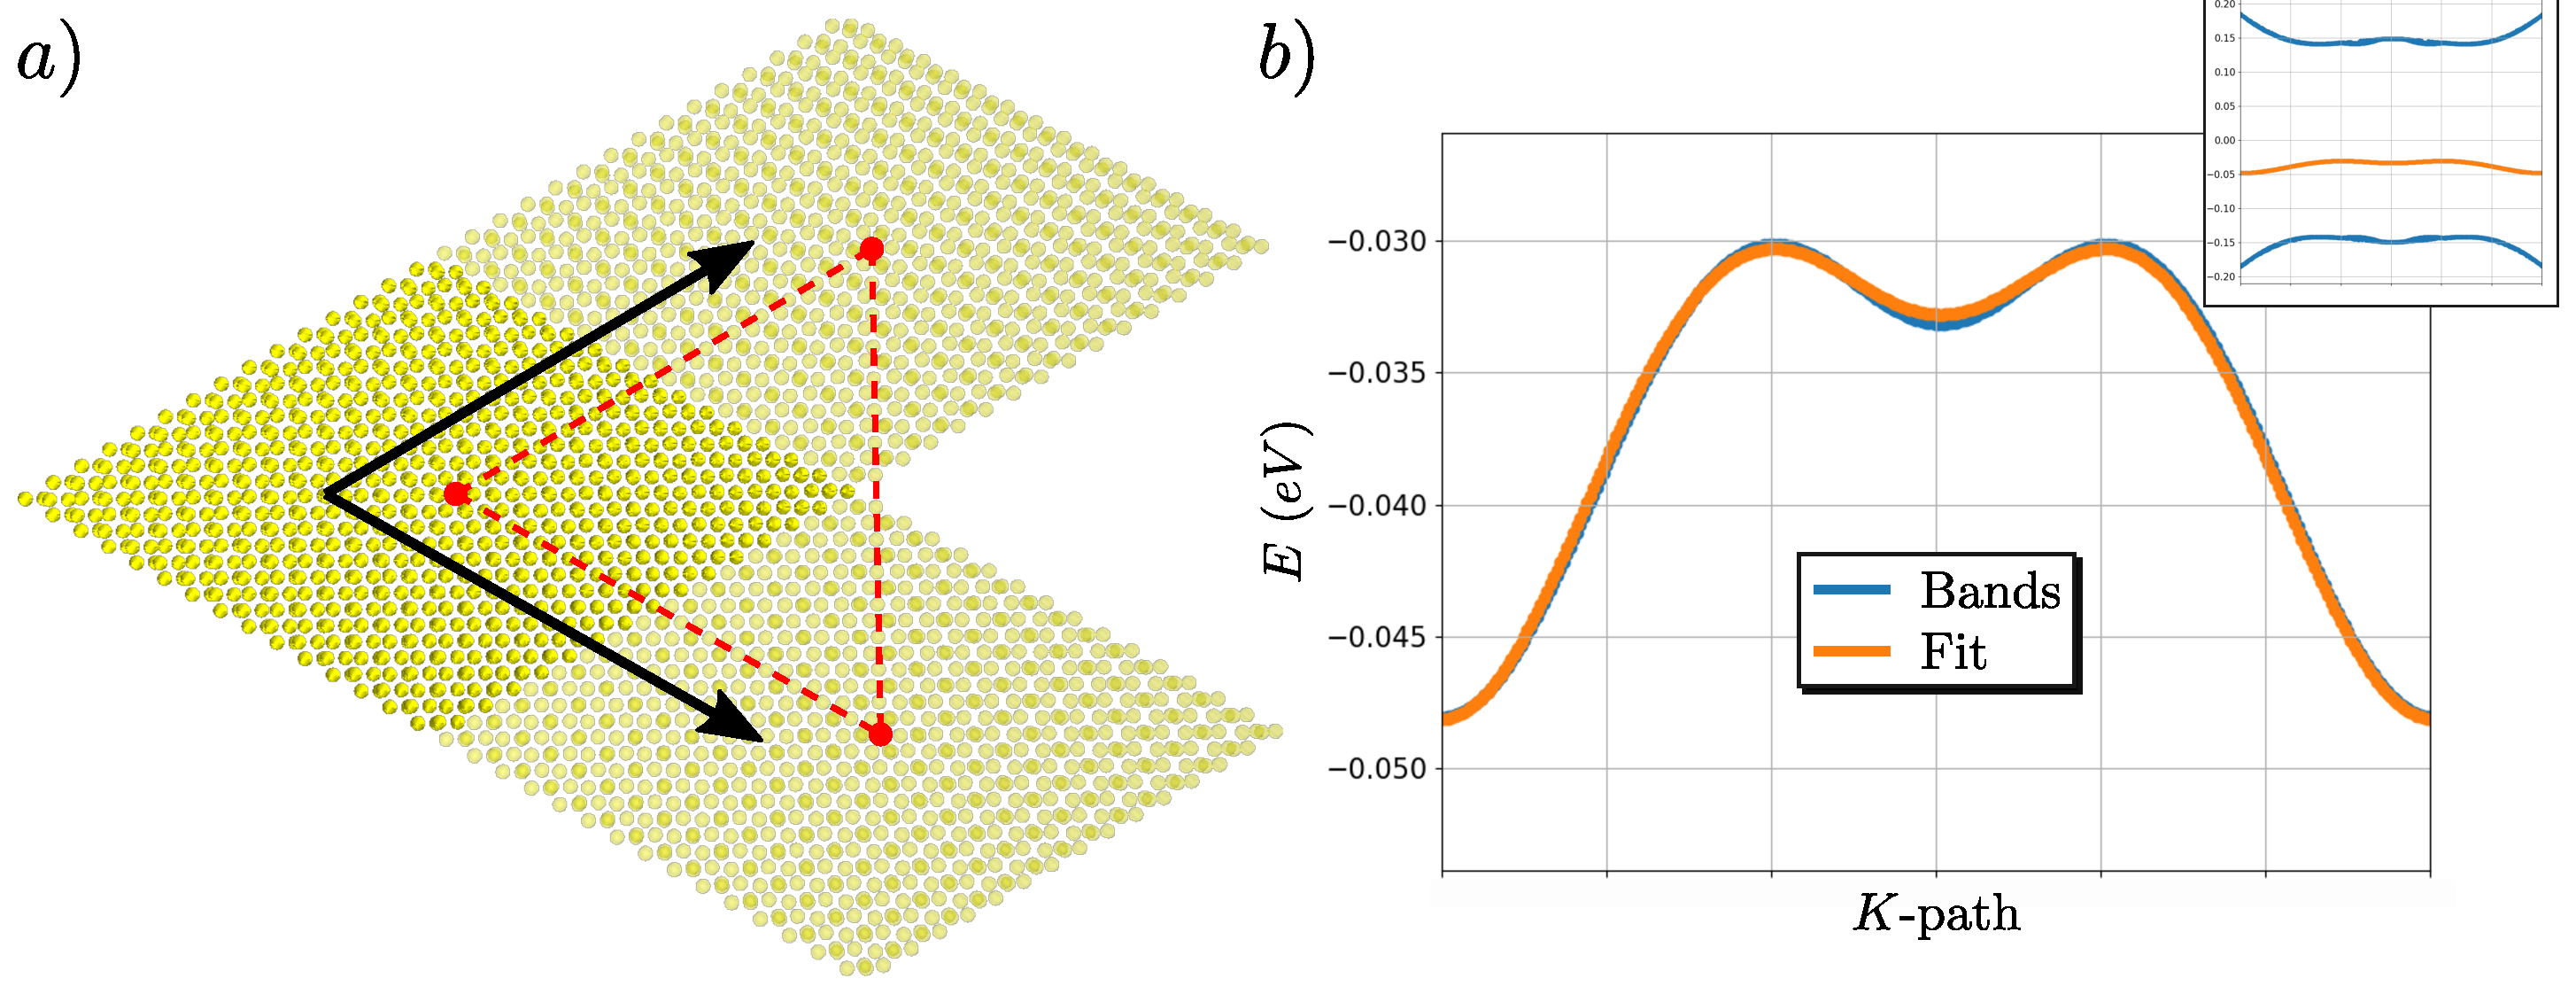
\includegraphics[width=0.8\textwidth]{artlat/fig/triangular_bands.pdf}
  \vspace{-5pt}
  \caption{$a)$ shows an example of a unit cell with the vacancies placed in such a way that the translational symmetry creates an artificial triangular lattice. $b)$ shows the in-gap bands (orange in the inset) that appear because of the vacancies, the fit is done using a model with up to third neighbors.}
  \label{triangular}
\end{figure}
\FloatBarrier
%~~~~~~~~~~~~~~~~~~~~~~~~~~~~~~~~~~~~~~~~~~~~~~~~~~~~~~~~~~~%

In Fig.~\ref{triangular} $a)$ we can be the architecture considered, a single vacancy in the center of the unit cell and the standard lattice vectors for a graphene supercell. The lattice of impurities form an in-gap band which resembles that of a triangular lattice.
In particular it can be fit to a model like:
\begin{equation}
\begin{split}
  H(k) = E_0 &+
         2t_1\left[ cos\left(\vec{k}\vec{a}_1\right) +
                    cos\left(\vec{k}\vec{a}_2\right) +
                    cos\left(\vec{k}(\vec{a}_1-\vec{a}_2)\right)
              \right] +\\
         &+2t_2\left[ cos\left(\vec{k}(\vec{a}_1+\vec{a}_2)\right) +
                    cos\left(\vec{k}(2\vec{a}_1-\vec{a}_2)\right) +
                    cos\left(\vec{k}(-\vec{a}_1+2\vec{a}_2)\right)
             \right] +\\
         &+2t_3\left[ cos\left(2\vec{k}\vec{a}_1\right) +
                    cos\left(2\vec{k}\vec{a}_2\right) +
                    cos\left(2\vec{k}(\vec{a}_1-\vec{a}_2)\right)
              \right]
\end{split}
\label{triangular_hamil}
\end{equation}
Where $\vec{k}$, $\vec{a}_1$ and $\vec{a}_2$ are the Bloch vector and the lattice vectors respectively. The parameters that best fit the model \eqref{triangular_hamil} are the following:
\begin{equation}
\begin{split}
  E_0 &= \SI{-0.036}{\eV}\\
  t_1 = \SI{-1.93e-3}{\eV} \quad;\quad
  t_2 &= \SI{7.40e-5}{\eV} \quad;\quad
  t_3 = \SI{-5.26e-5}{\eV}
\end{split}
\end{equation}


\section{Artificial graphene}
In order to create an artificial graphene crystal we need to place the vacancies at a particular distance that depends on the size of the chosen unit cell.
The basic unit cell and lattice vectors for graphene are
\begin{equation}
\begin{split}
  r_0 = a\left(-\frac{1}{2},0,0\right) \qquad ; \qquad
  r_1 = a\left(\frac{1}{2},0,0\right)\\
  a_1 = a\left(\frac{3}{2},\frac{\sqrt{3}}{2},0\right) \qquad ; \qquad
  a_2 = a\left(\frac{3}{2},-\frac{\sqrt{3}}{2},0\right)
\end{split}
\end{equation}
In order to separate the vacancies, bigger cells must be used, the lattice vectors will escalate for a cell of size $n$:
\begin{equation}
  \vec{a}^n_1 = n \vec{a}_1 \qquad ; \qquad \vec{a}^n_2 = n \vec{a}_2
\end{equation}
Since the vacancies have to be in the same sublattice, the possible distances for them are $d_v = 3na$, being $a=\SI{1.4}{\angstrom}$ the $C$-$C$ distance. The corresponding lattice vectors should be:
\begin{equation}
  \vec{a}^n_1 = 3na\left(\frac{3}{2},\frac{\sqrt{3}}{2},0\right) \qquad ; \qquad
  \vec{a}^n_2 = 3na\left(\frac{3}{2},-\frac{\sqrt{3}}{2},0\right)
\end{equation}
This simple relation shows that only supercells which are a multiple of 3 are feasible.


% Therefore a perfect graphene lattice will only emerge when $|\vec{a}^n_1|=|\vec{a}^n_2|=3na$. Notice that $m$ and $n$ are independent indices.
% \begin{equation}
%   |\vec{a}^n| = \sqrt{3}na \quad\Rightarrow n = \sqrt{3}m
% \end{equation}
% \red{Impossible?!}

When the vacancies are placed at that distance, and are properly oriented (see Fig~\ref{graphene}) the in-gap states interact among them forming two dispersing bands all over the Brillouin zone.
%~~~~~~~~~~~~~~~~~~~~~~~~~~ FIGURE ~~~~~~~~~~~~~~~~~~~~~~~~~%
\begin{figure}[h!]
  \centering
  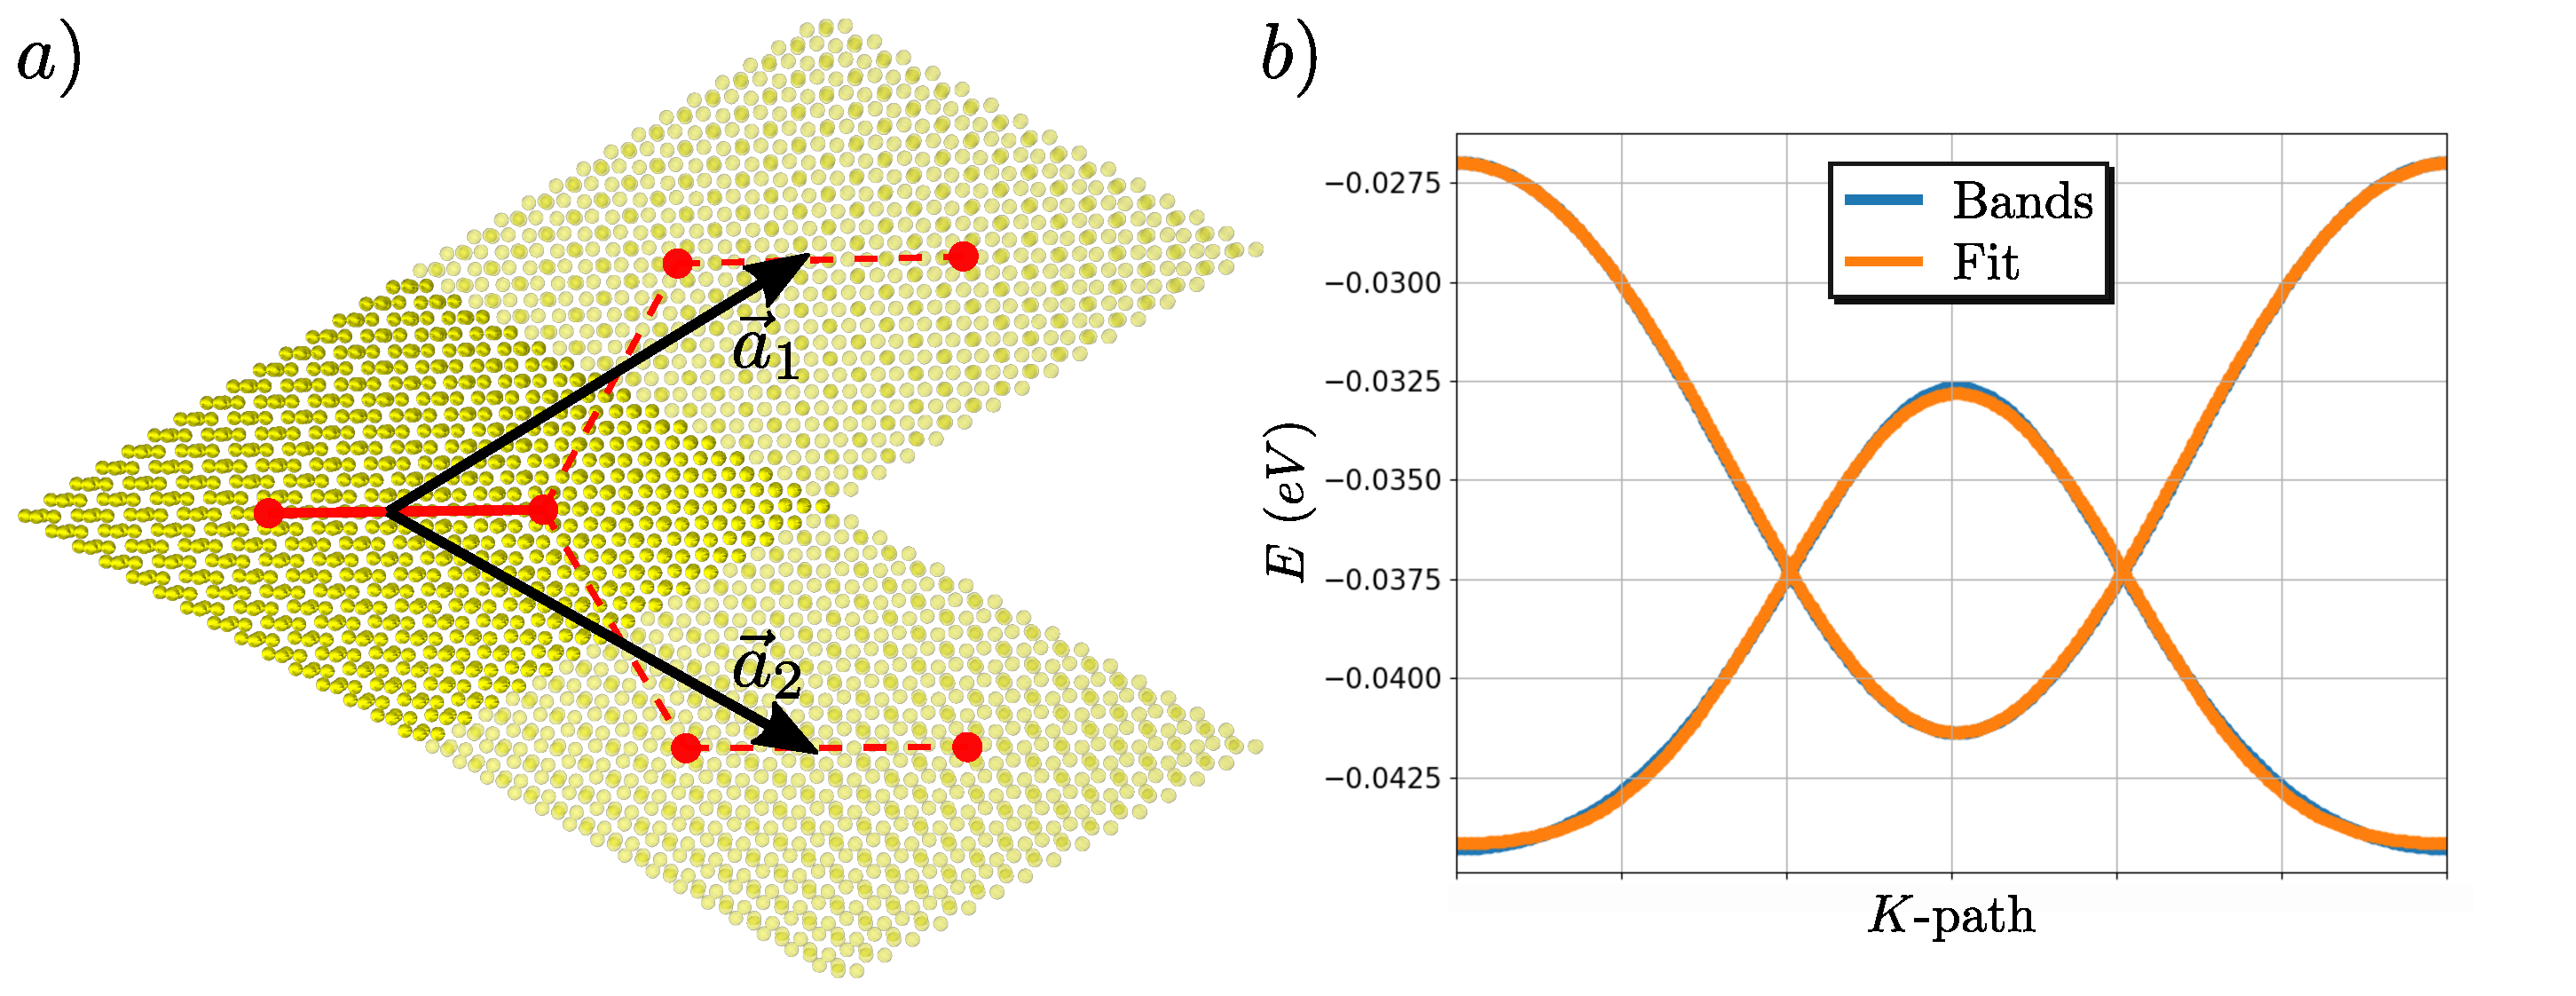
\includegraphics[width=0.8\textwidth]{artlat/fig/graphene_bands.pdf}
  \vspace{-5pt}
  \caption{$a)$ shows an example of a unit cell with the vacancies placed in such a way that the translational symmetry creates an artificial graphene lattice. $b)$ shows the in-gap bands (orange) that appear because of the vacancies, the fit is done using a model with up to third neighbors.}
  \label{graphene}
\end{figure}
\FloatBarrier
%~~~~~~~~~~~~~~~~~~~~~~~~~~~~~~~~~~~~~~~~~~~~~~~~~~~~~~~~~~~%
In Fig.~\ref{graphene} $b)$ we can see the dispersing in-gap bands as well as a fit of said bands to a simple model with up to third neighbors.

\begin{equation}
\begin{split}
  % E_0 = \SI{-0.03670772697798405}{\eV}
  % t_1 = \SI{-0.003216525825060562}{\eV}
  % t_2 = \SI{0.00018838793316003813}{\eV}
  % t_3 = \SI{0.0003533798537212944}{\eV}
  E_0 &= \SI{-0.037}{\eV}\\
  t_1 = \SI{-3.22e-3}{\eV} \quad;\quad
  t_2 &= \SI{1.88e-4}{\eV} \quad;\quad
  t_3 = \SI{3.53e-4}{\eV}
\end{split}
\end{equation}

%~~~~~~~~~~~~~~~~~~~~~~~~~~ FIGURE ~~~~~~~~~~~~~~~~~~~~~~~~~%
\begin{figure}[!ht!]
\centering
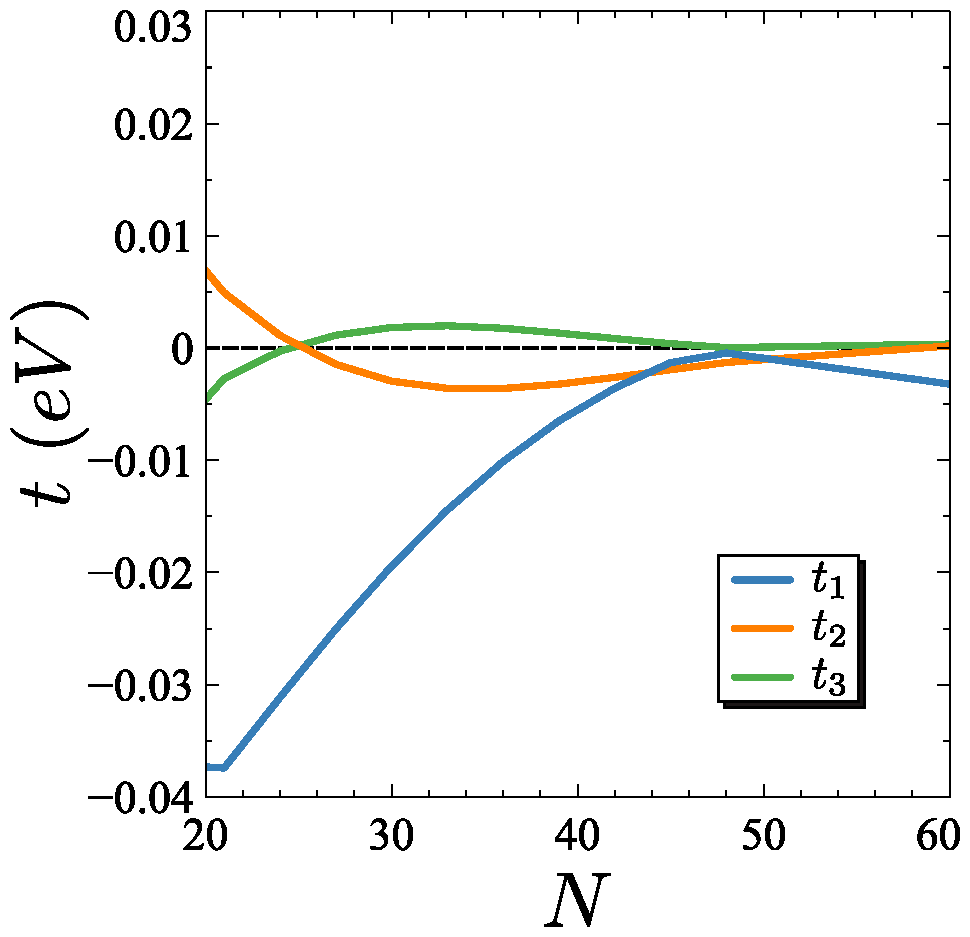
\includegraphics[width=0.5\textwidth]{artlat/fig/params.pdf}
\vspace{-5pt}
\caption{Evolution of the hopping parameters of a graphene tight-binding model with third neighbor hoppings.}
\label{hopp}
\end{figure}
\FloatBarrier
%~~~~~~~~~~~~~~~~~~~~~~~~~~~~~~~~~~~~~~~~~~~~~~~~~~~~~~~~~~~%






\section{Artificial Kagome}
the position of the adatoms to have an artificial Kagome lattice are:
\begin{equation}
  r_1 = \frac{a_k}{2}\left(\sqrt{3}/2,  0 ,0\right),\quad
  r_2 = \frac{a_k}{2}\left(-\sqrt{3}/2,1,0\right),\quad
  r_3 = \frac{a_k}{2}\left(-\sqrt{3}/2,-1,0\right)
\end{equation}

where $a_k = |a_1|/2$. This geometry only works regularly for odd supercells as seeing in Fig.~\ref{kagome}


%~~~~~~~~~~~~~~~~~~~~~~~~~~ FIGURE ~~~~~~~~~~~~~~~~~~~~~~~~~%
\begin{figure}[h!]
  \centering
  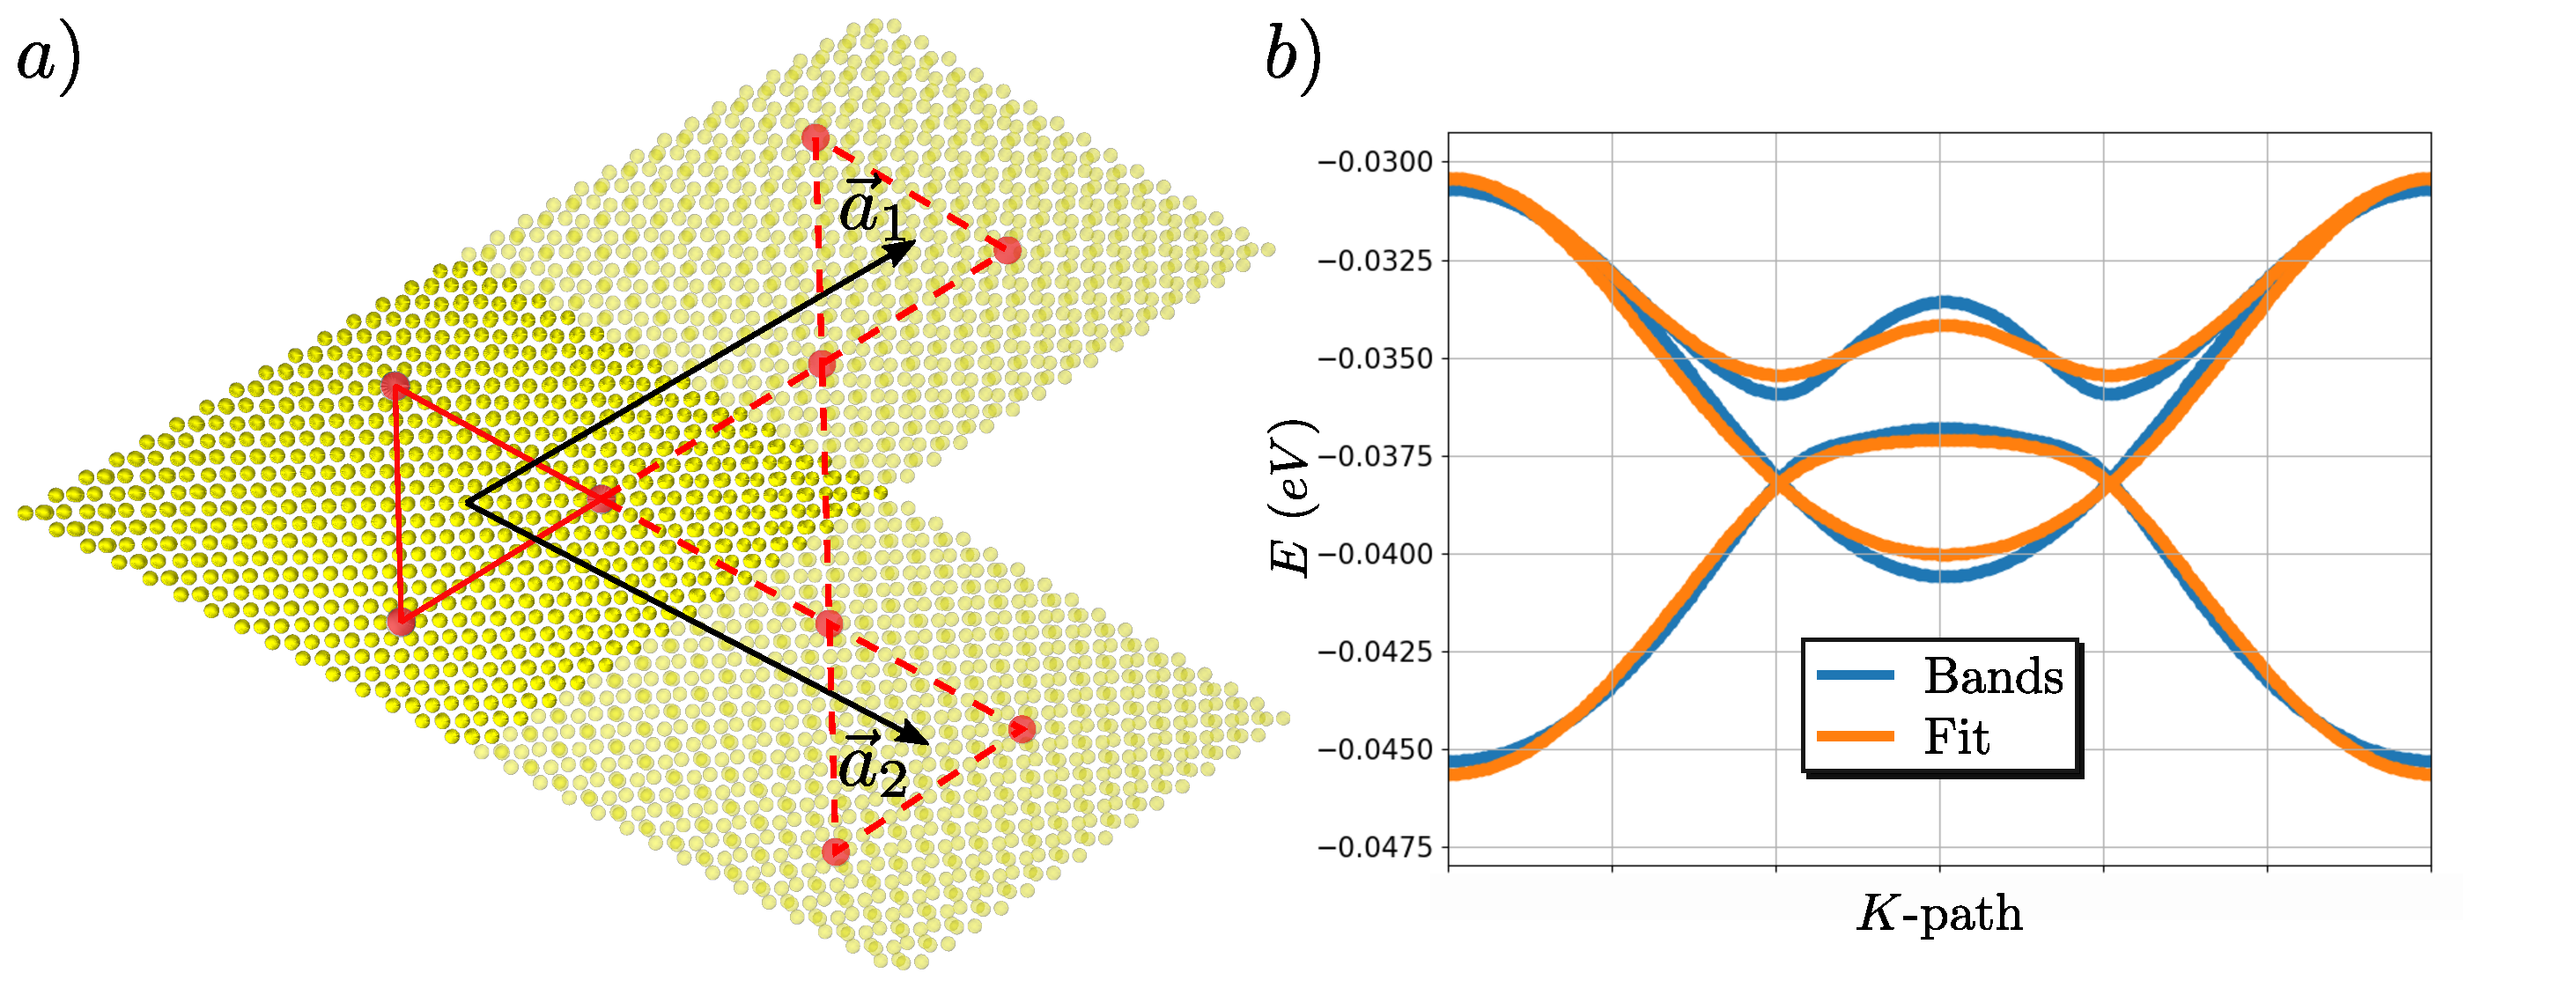
\includegraphics[width=0.8\textwidth]{artlat/fig/kagome_bands.pdf}
  \vspace{-5pt}
  \caption{$a)$ shows an example of a unit cell with the vacancies placed in such a way that the translational symmetry creates an artificial Kagome lattice. $b)$ shows the in-gap bands (orange) that appear because of the vacancies, the fit is done using a model with up to second neighbors.}
  \label{kagome}
\end{figure}
\FloatBarrier
%~~~~~~~~~~~~~~~~~~~~~~~~~~~~~~~~~~~~~~~~~~~~~~~~~~~~~~~~~~~%
\begin{equation}
\begin{split}
  % E_0 = -0.03669201703555982
  % t_1 = -0.002000033597883536
  % t_2 = -0.000536649553068988
  % t_3 = 0.00020143407845221853
  E_0 &= \SI{-0.037}{\eV}\\
  t_1 = \SI{-2.00e-3}{\eV} \quad;\quad
  t_2 &= \SI{-5.37e-4}{\eV} \quad;\quad
  t_3 = \SI{2.01e-4}{\eV}
\end{split}
\end{equation}
A geometric cheat sheet can be found in appendix~\ref{models}





\section{Parameters control. Hubbard dimer}

In order to determine the ground state as a function of both the electric field $\mathcal{E}$ and the distance between vacancies $d$ we use the fact that the spectrum of the blue Hamiltonian looks like one of the structures shown in Fig.~\ref{spectrum_dimer}. Considering the standard deviation of the 3 lowest eigenvalues (0-2), and the same quantity skipping one eigenvalue (1-3) we can obtain a quantity that will flip sign if the singlet and triplet cross.

%~~~~~~~~~~~~~~~~~~~~~~~~~~ FIGURE ~~~~~~~~~~~~~~~~~~~~~~~~~%
\begin{figure}[h!]
\centering
  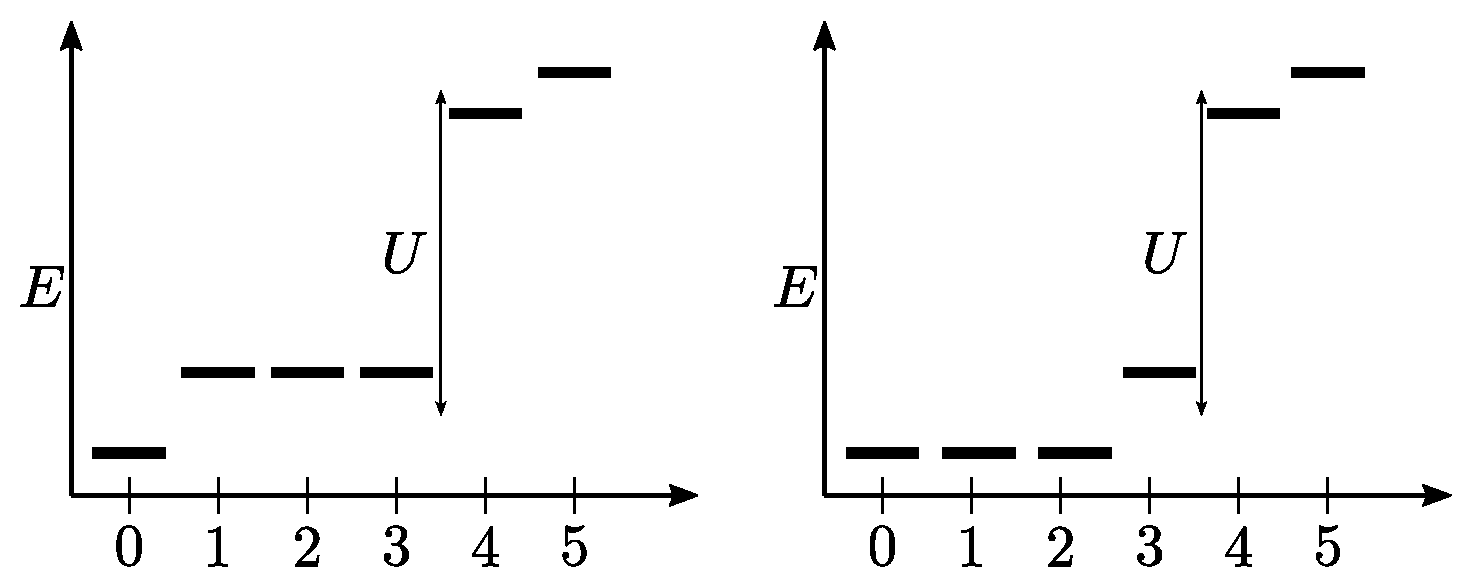
\includegraphics[width=0.7\textwidth]{artlat/fig/sketch_levels.pdf}
\vspace{-5pt}
\caption{Possible structure of the spectrum of the eigenvalues of the blue Hamiltonian.}
\label{spectrum_dimer}
\end{figure}
\FloatBarrier
%~~~~~~~~~~~~~~~~~~~~~~~~~~~~~~~~~~~~~~~~~~~~~~~~~~~~~~~~~~~%

%~~~~~~~~~~~~~~~~~~~~~~~~~~ FIGURE ~~~~~~~~~~~~~~~~~~~~~~~~~%
\begin{figure}[h!]
\centering
  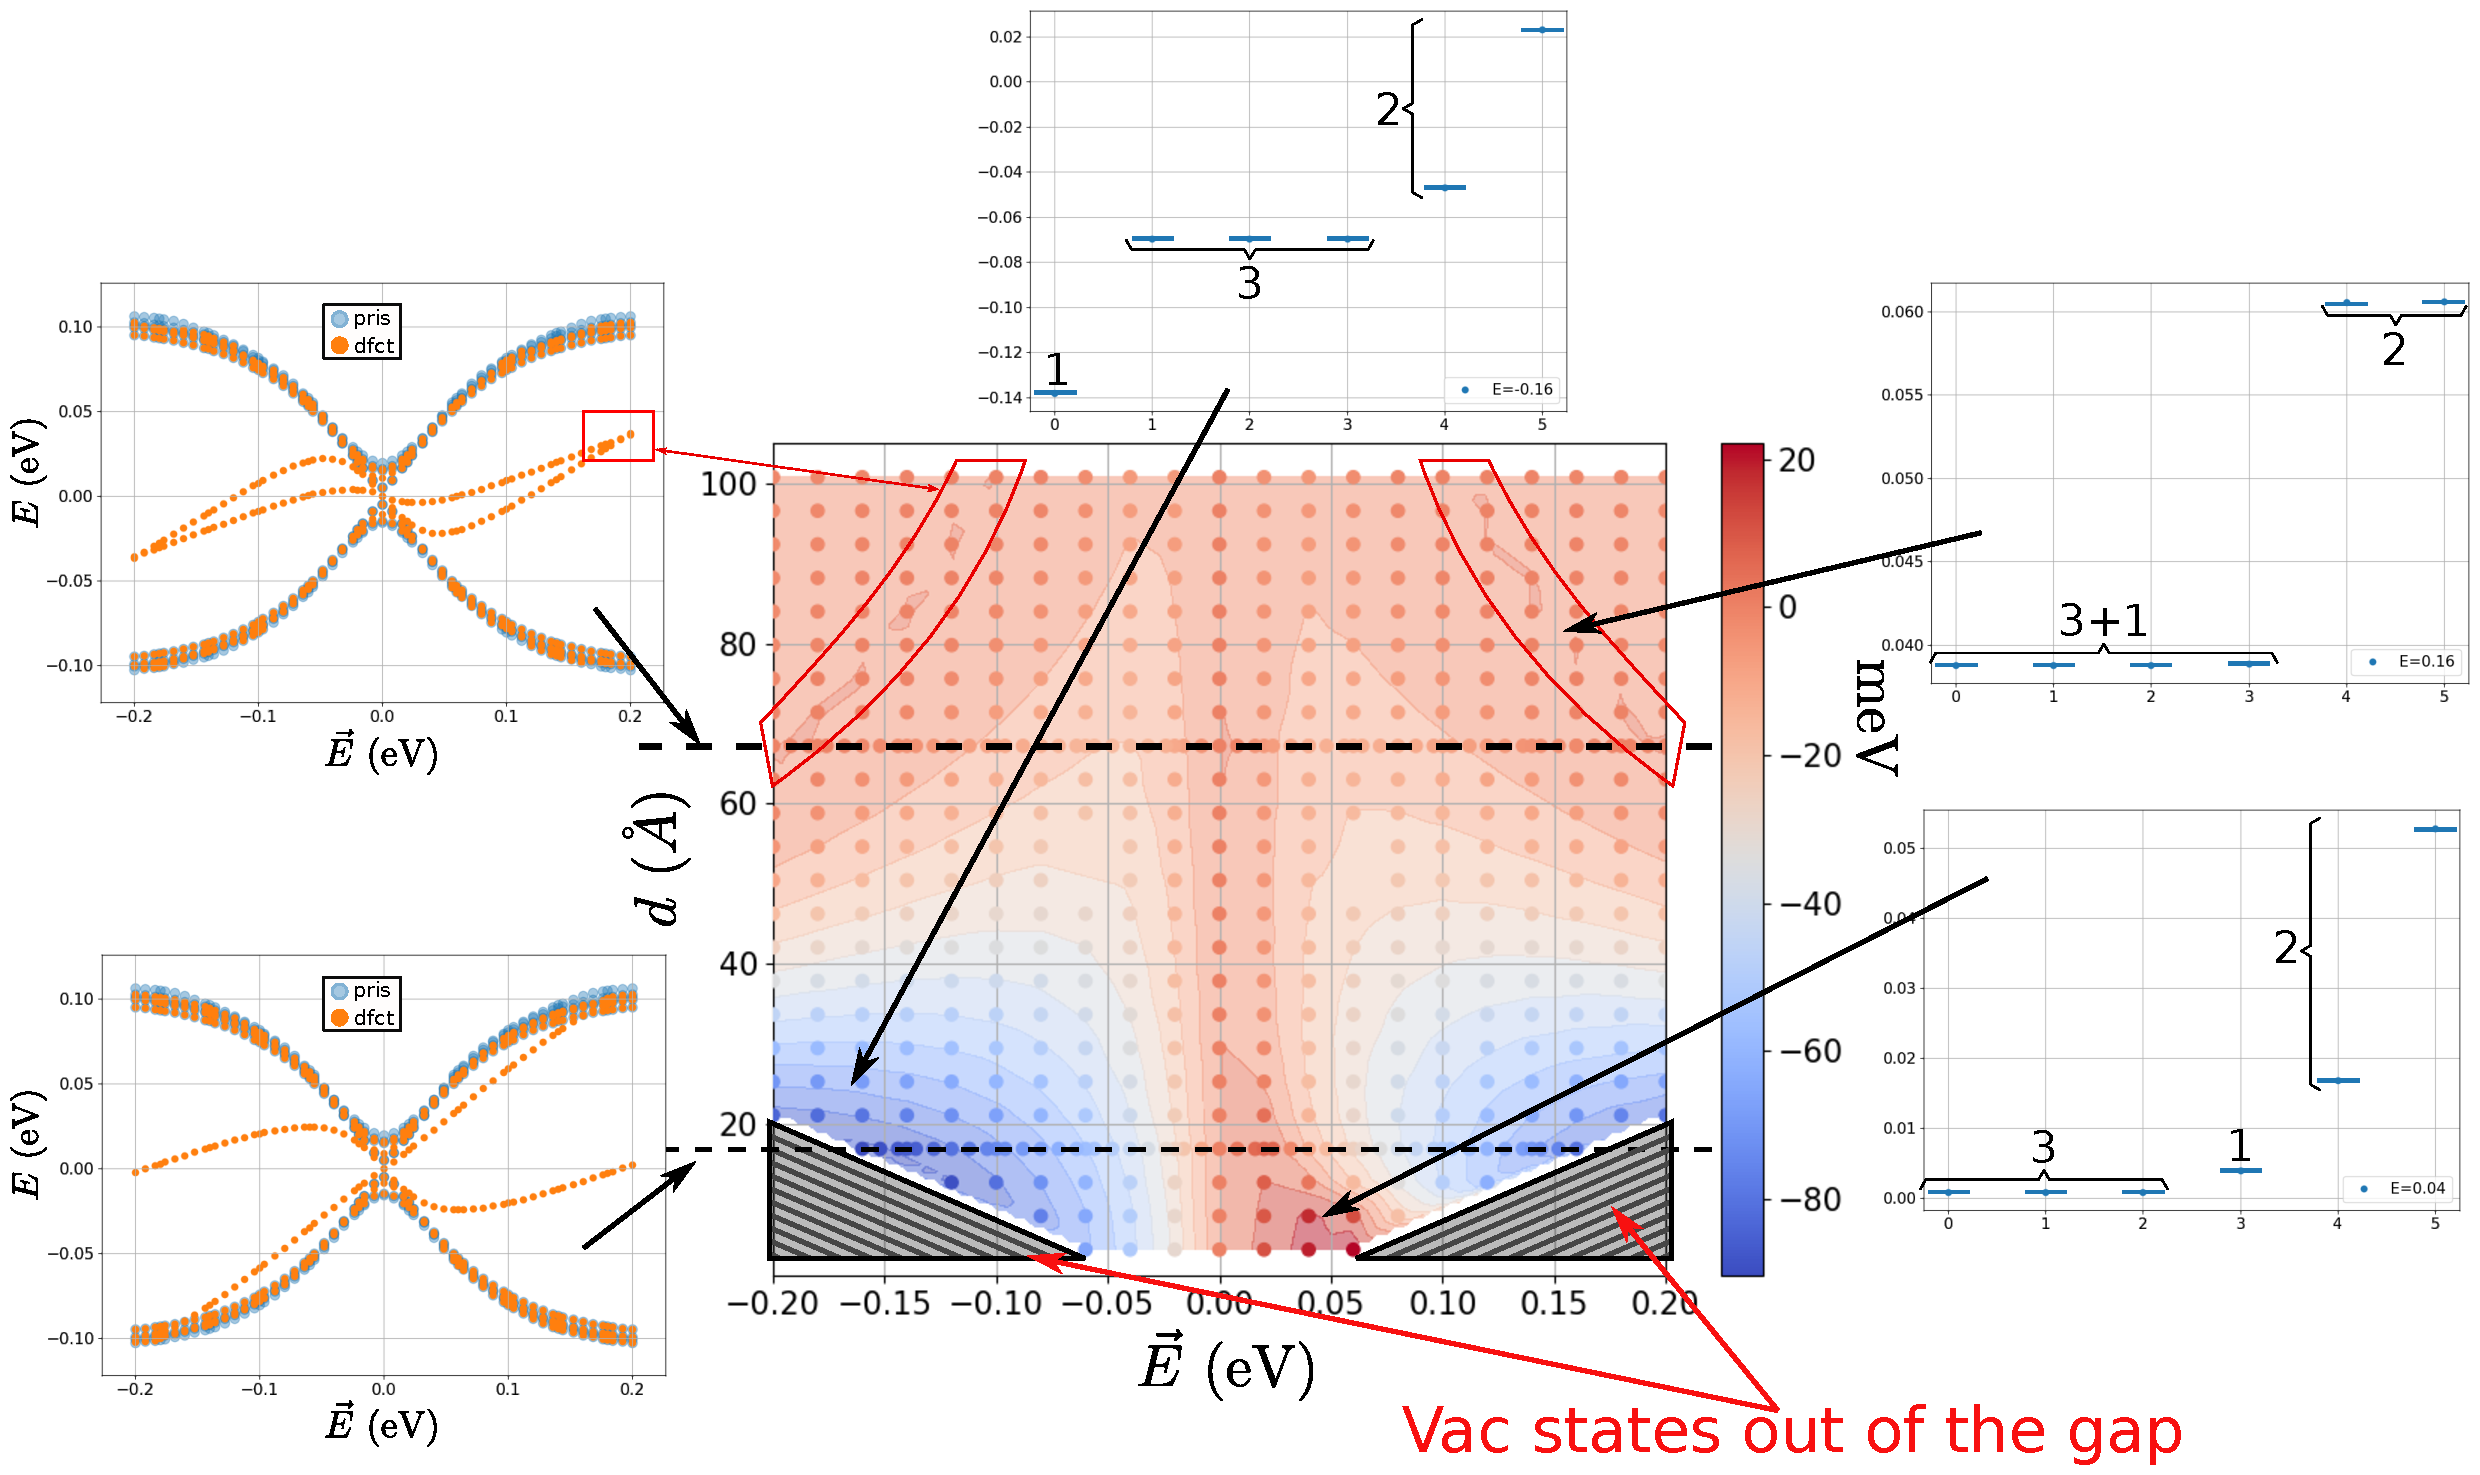
\includegraphics[width=0.7\textwidth]{artlat/fig/phase_J.pdf}
\vspace{-5pt}
\caption{Phase space showing the arrangement of the ground state as exposed in the text}
\label{}
\end{figure}
\FloatBarrier
%~~~~~~~~~~~~~~~~~~~~~~~~~~~~~~~~~~~~~~~~~~~~~~~~~~~~~~~~~~~%

%~~~~~~~~~~~~~~~~~~~~~~~~~~ FIGURE ~~~~~~~~~~~~~~~~~~~~~~~~~%
\begin{figure}[h!]
\centering
  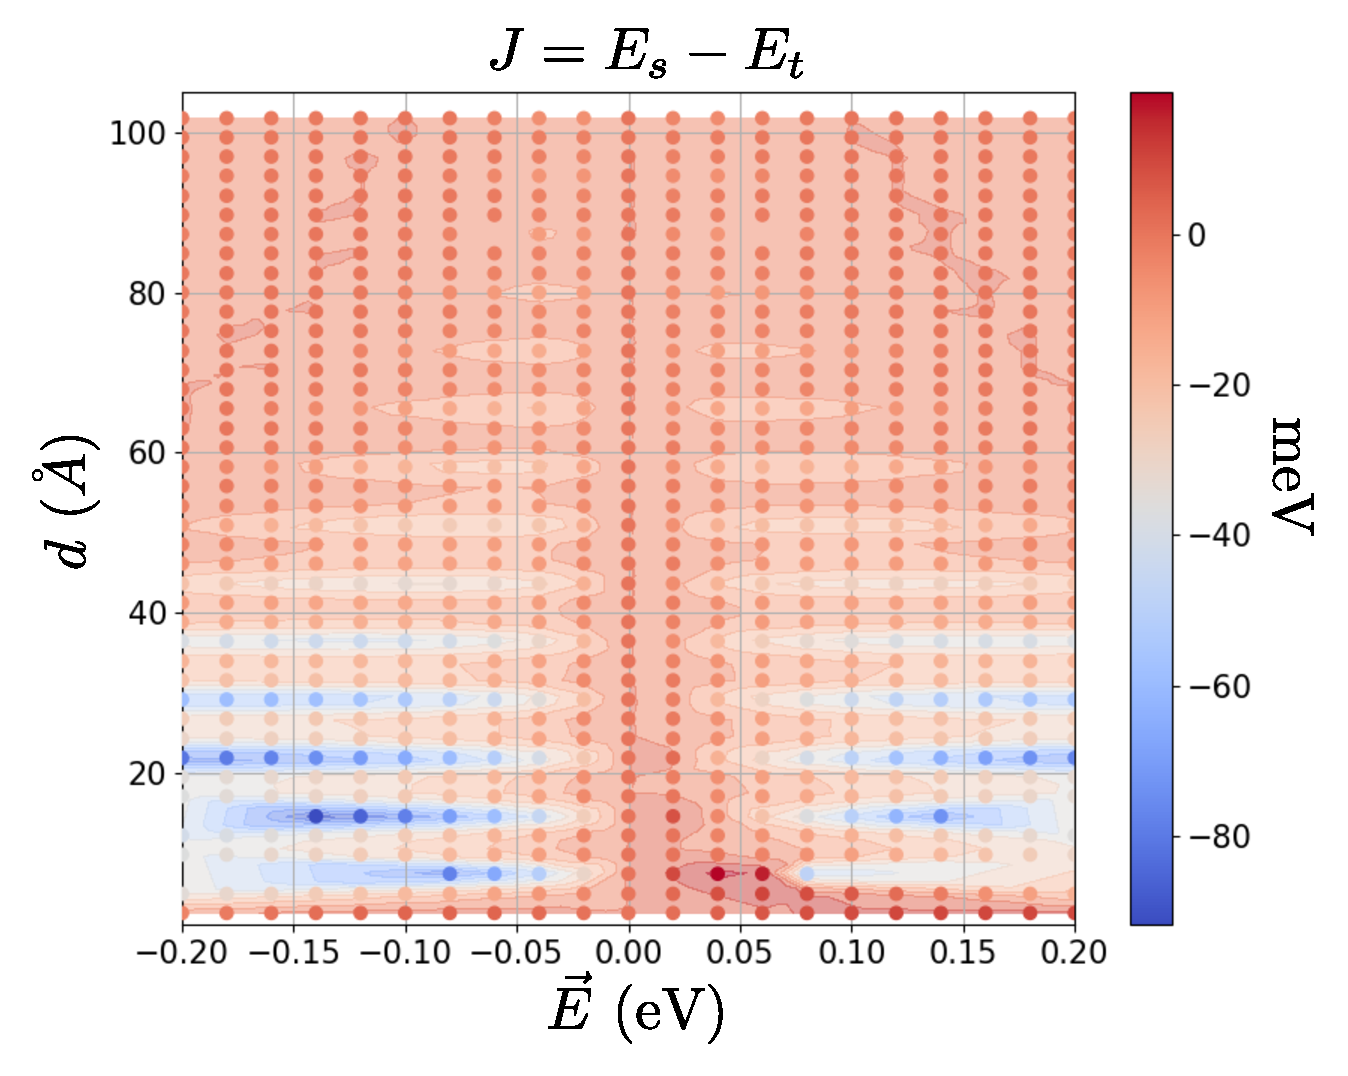
\includegraphics[width=0.7\textwidth]{artlat/fig/phase_J30.pdf}
\vspace{-5pt}
\caption{Phase space showing the arrangement of the ground state as exposed in the text for $\alpha=30$}
\label{}
\end{figure}
\FloatBarrier
%~~~~~~~~~~~~~~~~~~~~~~~~~~~~~~~~~~~~~~~~~~~~~~~~~~~~~~~~~~~%

